
\begin{exercice}[Un peu de vocabulaire]
Recopie et complète les phrases en utilisant les mots « côtés », « sommets », « diagonales », « opposés » et « consécutifs ».\\[-3em]
\begin{minipage}[c]{0.26\linewidth}
\vspace{2cm}
 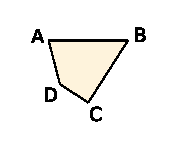
\includegraphics[width=2cm]{quad_rose}
 \end{minipage} \hfill%
 \begin{minipage}[t]{0.66\linewidth}
 Dans le quadrilatère $ABCD$ :
 \begin{enumerate}
  \item $[AB]$ et $[CD]$ sont des \ldots \ldots \ldots ;
  \item $C$ et $D$ sont des \ldots \ldots \ldots ;
  \item $[AD]$ et $[BC]$ sont des \ldots \ldots \ldots ;
  \item $[AC]$ et $[BD]$ sont les \ldots \ldots \ldots ;
  \item $A$ et $C$ sont des \ldots \ldots \ldots ;
  \item $[AB]$ et $[BC]$ sont des \ldots \ldots \ldots .
  \end{enumerate}
 \end{minipage} \\
\end{exercice}

%%%%%%%%%%%%%%%%%%%%%%%%%%%%%%%%%%%%%%%%%%%%%%%%%%%%%%%%%%%%%%%%%

\serie{parallélogrammes}


\begin{exercice}
Construis les parallélogrammes donnés par leur croquis dont les mesures sont données en cm. Dans chacun des cas, précise quelle propriété a été utilisée pour la construction :
\begin{colenumerate}{2}
 \item
 
 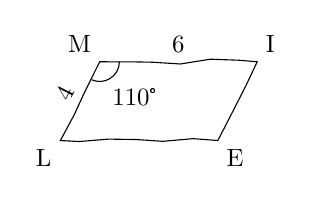
\begin{tikzpicture}[rotate=0,every node/.style={scale=0.9},scale=0.5]

\coordinate (M) at (0,0);
\coordinate (I) at (4,0);
\coordinate (E) at (3,-2);
\coordinate (L) at (-1,-2);

\draw[decorate,decoration={random steps,amplitude=1pt,segment length=10pt}] (M) node [above left]{M}--(I) node [above right]{I}--(E) node [below right] {E}--(L) node [below left] {L}--cycle;

\draw (0.5,0) arc (0:-114:0.5);
\node at (0.9,-0.9){110°};

\path (M)--(L) node[midway,above,sloped]{4};
\path (M)--(I) node[midway,above]{6};
\end{tikzpicture}
  \item
 
 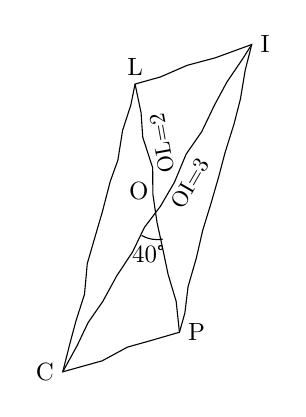
\begin{tikzpicture}[rotate=60,every node/.style={scale=0.9},scale=0.8]

\coordinate (C) at (0,0);
\coordinate (L) at (4.53,1.29);
\coordinate (I) at (6,0);
\coordinate (P) at (1.47,-1.29);
\coordinate (O) at (3,0); %le centre du parallélogramme

\draw[decorate,decoration={random steps,amplitude=1pt,segment length=10pt}] (C) node [left]{C}--(L) node [above]{L}--(I) node [right] {I}--(P) node [right] {P}--cycle;

\draw [decorate,decoration={random steps,amplitude=1pt,segment length=10pt}] (C)--(I) (L)--(P);
\draw (2.5,0) arc (-180:-140:0.5);
\draw (2.3,-0.25) node {40°};
\draw (O) node [above left]{O};

\path (O)--(I) node[pos=0.2,below,sloped,scale=0.9,rotate=60]{OI=3};
\path (O)--(L) node[midway,below,sloped,scale=0.9,rotate=60]{OL=2};

\end{tikzpicture}


  \item
 
 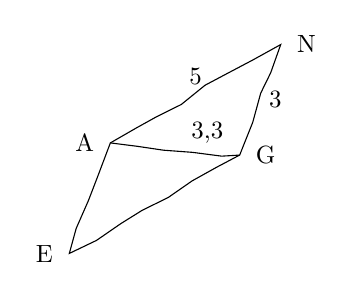
\begin{tikzpicture}[rotate=30,every node/.style={scale=0.9},scale=0.5]

\coordinate (A) at (0,0);
\coordinate (N) at (5,0);
\coordinate (G) at (2.69,-1.91);
\coordinate (E) at (-2.31,-1.91);

\draw[decorate,decoration={random steps,amplitude=1pt,segment length=10pt}] (A) node [left=3pt]{A}--(N) node [right=3pt]{N}--(G) node [right=3pt] {G}--(E) node [left=3pt] {E}--cycle;
\draw [decorate,decoration={random steps,amplitude=1pt,segment length=10pt}] (A)--(G);
\path (A)--(N) node[midway,above]{5};
\path (N)--(G) node[midway,right]{3};
\path (A)--(G) node[near end,above]{3,3};

\end{tikzpicture}
  \item
 
 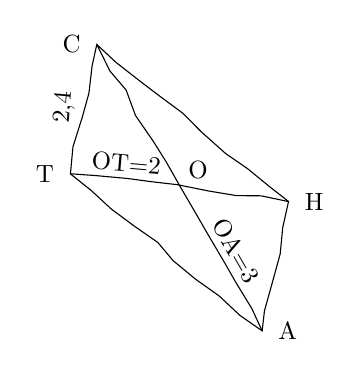
\begin{tikzpicture}[rotate=-60,every node/.style={scale=0.9},scale=0.7]

\coordinate (C) at (0,0);
\coordinate (H) at (4.21,1.59);
\coordinate (A) at (6,0);
\coordinate (T) at (1.79,-1.59);
\coordinate (O) at (3,0); %le centre du parallélogramme

\draw[decorate,decoration={random steps,amplitude=1pt,segment length=10pt}] (C) node [left=3pt]{C}--(H) node [right=3pt]{H} --(A) node [right=3pt] {A}--(T) node [left=3pt] {T}--cycle;
\draw [decorate,decoration={random steps,amplitude=1pt,segment length=10pt}] (C)--(A) (H)--(T);
\node at (O)[above right]{O}; 
\node at (4.5,0)[above,rotate=-60]{OA=3};
\path (C)--(T) node[midway,above,rotate=85]{2,4};
\path (T)--(O) node[midway,above,rotate=-5]{OT=2};

\end{tikzpicture}

 \end{colenumerate}
\end{exercice}


\begin{exercice}
Lorsque c'est possible, construis les parallélogrammes $ABCD$ suivants. Quand la construction n'est pas possible, explique pourquoi :
\begin{enumerate}
 \item $AB = 5$ cm, $AD = 3,5$ cm et $BD = 7$ cm ;
 \item $AB = 2$ cm, $AD = 4,5$ cm et $BD= 3,5$ cm ;
 \item $AD = 4$ cm, $AB = 2,8$ cm et $BD = 7$ cm ;
 \item Construis un carré $IJKL$ tel que $IK = 6,4$ cm.
 \end{enumerate}
\end{exercice}


\begin{exercice}
Pour chacun des parallélogrammes suivants, fais d’abord un croquis puis construis :
\begin{enumerate}
 \item $VERT$ avec $VT = 5$ cm, $\widehat{ERT} = 125^\circ$ et $VE = 4$ cm ;
 \item $BLEU$ de centre $I$ avec $BL = 6$ cm, $UI = 3$ cm et $IE = 4$ cm ;
 \item $NOIR$ avec $NI = 62$ mm, $\widehat{NIR} = 40^\circ$ et $\widehat{RNI} = 30^\circ$.  
 \end{enumerate}
\end{exercice}

\begin{exercice}
Trace un segment $[GR]$ de 7 cm. Construis un parallélogramme dont $[GR]$ est un côté puis un autre dont $[GR]$ est une diagonale.
\end{exercice}


\begin{exercice}[Avec trois points]
\begin{enumerate}
 \item Place trois points $P$, $I$ et $M$ tels que le segment $PI = 4$ cm, le segment $IM = 5$ cm et l'angle $\widehat{PIM} = 130^\circ$ ;
 \item Trouve tous les points $N$ $(N_1, N_2, \ldots)$ tels que les points $P$, $I$, $M$ et $N$ soient les sommets d'un parallélogramme.
 \end{enumerate}
\end{exercice}




%%%%%%%%%%%%%%%%%%%%%%%%%%%%%%%%%%%%%%%%%%%%%%%%%%%%%%%%%%%%%%%%%

\serie{losanges}


\begin{exercice}
Construis les losanges donnés par leur croquis dont les mesures sont données en cm :
\begin{colenumerate}{2}
 \item
 
  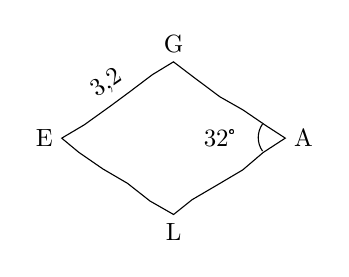
\begin{tikzpicture}[rotate=0,every node/.style={scale=0.9}]

\coordinate (E) at (0,0);
\coordinate (G) at (1.42,0.97);
\coordinate (A) at (2.84,0);
\coordinate (L) at (1.42,-0.97);



\draw[decorate,decoration={random steps,amplitude=1pt,segment length=10pt}] (E) node [left]{E}--(G) node [above]{G}--(A) node [right] {A}--(L) node [below] {L}--cycle;

\draw (2.55,0.18) arc (145:215:0.3) node [midway, left=5pt] {32°};
\path (E)--(G) node[midway,above,sloped]{3,2};
\end{tikzpicture}
  \item
 
 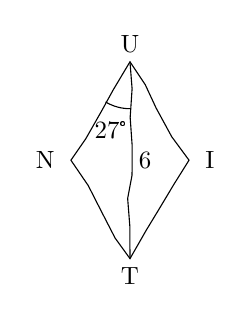
\begin{tikzpicture}[rotate=0,every node/.style={scale=0.9},scale=1]

\coordinate (N) at (0,0);
\coordinate (U) at (0.75,1.25);
\coordinate (I) at (1.5,0);
\coordinate (T) at (0.75,-1.25);

\draw[decorate,decoration={random steps,amplitude=1pt,segment length=10pt}] (N) node [left=3pt]{N}--(U) node [above]{U}--(I) node [right=3pt] {I}--(T) node [below] {T}--cycle;
\draw [decorate,decoration={random steps,amplitude=1pt,segment length=10pt}] (U)--(T);
\path (U)--(T) node[midway,right]{6};
\draw (0.44,0.74) arc (-120.96:-90:0.6) node[near start, below=3pt]{27°};

\end{tikzpicture}
  \item
 
   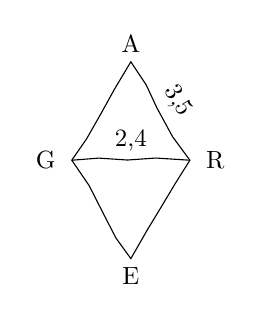
\begin{tikzpicture}[rotate=0,every node/.style={scale=0.9},scale=1]

\coordinate (G) at (0,0);
\coordinate (A) at (0.75,1.25);
\coordinate (R) at (1.5,0);
\coordinate (E) at (0.75,-1.25);

\draw[decorate,decoration={random steps,amplitude=1pt,segment length=10pt}] (G) node [left=3pt]{G}--(A) node [above]{A}--(R) node [right=3pt] {R}--(E) node [below] {E}--cycle;
\draw [decorate,decoration={random steps,amplitude=1pt,segment length=10pt}] (G)--(R);
\path (A)--(R) node[midway,above,sloped]{3,5};
\path (G)--(R) node[midway,above]{2,4};

\end{tikzpicture}
  \item
 
   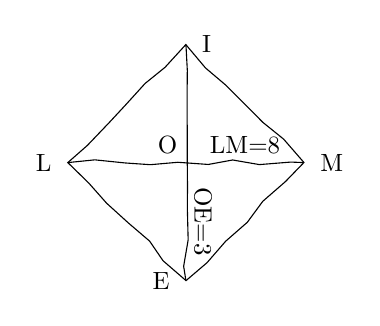
\begin{tikzpicture}[rotate=0,every node/.style={scale=0.9},scale=1]

\coordinate (L) at (0,0);
\coordinate (I) at (1.5,1.5);
\coordinate (M) at (3,0);
\coordinate (E) at (1.5,-1.5);
\coordinate (O) at (1.5,0); %le centre du losange

\draw[decorate,decoration={random steps,amplitude=1pt,segment length=10pt}] (L) node [left=3pt]{L}--(I) node [right=3pt]{I} --(M) node [right=3pt] {M}--(E) node [left=3pt] {E}--cycle;
\draw [decorate,decoration={random steps,amplitude=1pt,segment length=10pt}] (L)--(M) (I)--(E);
\node at (O)[above left]{O}; 
\path (O)--(E) node[midway,above,sloped]{OE=3};
\path (O)--(M) node[midway,above]{LM=8};
\end{tikzpicture}

 \end{colenumerate}
\end{exercice}


\begin{exercice}[Losanges]
\begin{enumerate}
 \item Construis un losange $ABCD$ avec $AB = 4$ cm ; \label{Quadrilateres_entrain}
 \item Sur du papier calque, construis un losange $A'B'C'D'$ tel que $A'B' = 4$ cm et $B'D' = 3,2$ cm.
 
Par superposition, compare cette figure avec celle de la question \ref{Quadrilateres_entrain} ;
 \item Construis un losange $EFGH$ tel que $EF = 32$ mm et $EG = 48$ mm.
 \end{enumerate}
\end{exercice}


\begin{exercice}
Dans chacun des cas suivants, construis un losange $LONG$ tel que :
\begin{enumerate}
 \item $\widehat{OLG} = 31^\circ$ et $LO = 3$ cm ;
 \item $\widehat{LON} = 131^\circ$ et $LO = 3$ cm ;
 \item $\widehat{OLN} = 31^\circ$ et $LO = 3$ cm.
 \end{enumerate}
\end{exercice}


\begin{exercice}[Mon beau losange]
Un professeur demande à trois élèves d'expliquer les différentes étapes pour construire un losange : 
\begin{itemize}
 \item Arnaud dit qu'il trace en pointillés un segment puis fait deux triangles isocèles identiques de chaque côté ;
 \item Sébastien dit qu'il trace en pointillés deux segments perpendiculaires qui se coupent en leur milieu puis qu'il relie leurs extrémités ;
 \item Audrey dit qu'elle trace deux segments de même longueur avec la même extrémité puis qu'elle trace les parallèles à ces deux segments.
 \end{itemize}
 \begin{enumerate}
  \item Pour chaque réponse d'élève, énonce la propriété du losange qui sert à sa construction.
  \item Construis les trois losanges en respectant les programmes de construction de chacun.
 \end{enumerate}
\end{exercice}


%%%%%%%%%%%%%%%%%%%%%%%%%%%%%%%%%%%%%%%%%%%%%%%%%%%%%%%%%%%%%%%%%

\serie{Rectangles}

\begin{exercice}[Des rectangles]
Dans chaque cas, fais d’abord un croquis puis construis :
\begin{enumerate}
 \item $LOUP$ est un rectangle tel que 
 
 $LO = 8$ cm et $LP = 6$ cm ;
 \item $NUIT$ est un rectangle tel que 
 
 $UI = 95$ mm et $IT = 112$ mm.
 \end{enumerate}
\end{exercice}
 
 
\begin{exercice}[D'autres rectangles]
\begin{enumerate}
 \item Construis un rectangle $ABCD$ tel que 
 
 $AB = 7,5$ cm et $AD = 4,8$ cm ;
 \item Construis des points $E$ et $F$ tels que 
 
 $DBEF$ soit un rectangle et $BE = 5$ cm ;
 \item Construis un rectangle $GRIS$ tel que 
 
 $GR = 9$ cm et $GI = 12$ cm ;
 \item Construis un rectangle $LUNE$ tel que 
 
 $LU = 0,6$ dm et $LN = 76$ mm.
 \end{enumerate} 
\end{exercice}


\begin{exercice}
Construis les rectangles donnés par leur croquis dont les mesures sont données en cm :
\begin{colenumerate}{2}
 \item
 
  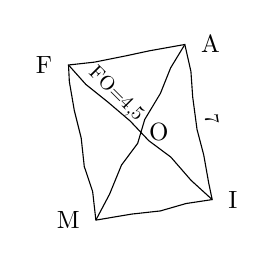
\begin{tikzpicture}[rotate=10,every node/.style={scale=0.9},scale=1]

\coordinate (F) at (0,0);
\coordinate (A) at (1.5,0);
\coordinate (I) at (1.5,-2);
\coordinate (M) at (0,-2);
\coordinate (O) at (0.75,-1); %le centre du rectangle

\draw[decorate,decoration={random steps,amplitude=1pt,segment length=10pt}] (F) node [left=3pt]{F}--(A) node [right=3pt]{A} --(I) node [right=3pt] {I}--(M) node [left=3pt] {M}--cycle;
\draw [decorate,decoration={random steps,amplitude=1pt,segment length=10pt}] (F)--(I) (A)--(M);
\node at (O)[right]{O}; 
\node at (.53,-.47)[rotate=-45,scale=0.8]{FO=4,5};
\path (A)--(I) node[midway,above,rotate=-80,scale=0.8]{7};
%\path (T)--(O) node[midway,above,rotate=-5]{OT=2};

\end{tikzpicture}

  \item
 
   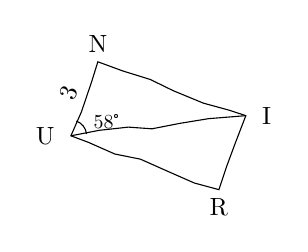
\begin{tikzpicture}[rotate=-20,every node/.style={scale=0.9},scale=1]

\coordinate (U) at (0,0);
\coordinate (N) at (0,1);
\coordinate (I) at (2,1);
\coordinate (R) at (2,0);

\draw[decorate,decoration={random steps,amplitude=1pt,segment length=10pt}] (U) node [left=3pt]{U}--(N) node [above]{N}--(I) node [right=3pt] {I}--(R) node [below] {R}--cycle;
\draw [decorate,decoration={random steps,amplitude=1pt,segment length=10pt}] (U)--(I);
\path (U)--(N) node[midway,above,rotate=70]{3};
\draw (0,0.2) arc (90:26.57:0.2) node[above=5pt,right,scale=0.8]{58°};

\end{tikzpicture}
  \item
 
   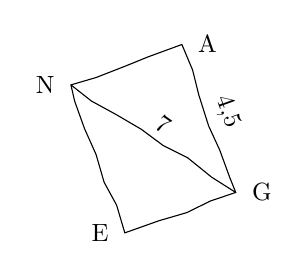
\begin{tikzpicture}[rotate=20,every node/.style={scale=0.9},scale=1]

\coordinate (N) at (0,0);
\coordinate (A) at (1.5,0);
\coordinate (G) at (1.5,-2);
\coordinate (E) at (0,-2);
\coordinate (O) at (0.75,-1); %le centre du rectangle

\draw[decorate,decoration={random steps,amplitude=1pt,segment length=10pt}] (N) node [left=3pt]{N}--(A) node [right=3pt]{A} --(G) node [right=3pt] {G}--(E) node [left=3pt] {E}--cycle;
\draw [decorate,decoration={random steps,amplitude=1pt,segment length=10pt}] (N)--(G);
\node at (.75,-1)[above,rotate=-35]{7};
\path (A)--(G) node[midway,above,rotate=-70]{4,5};

\end{tikzpicture}

  \item
 
   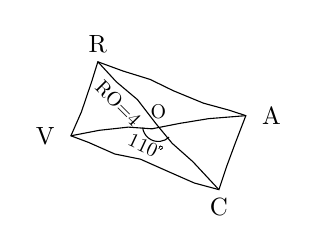
\begin{tikzpicture}[rotate=-20,every node/.style={scale=0.9},scale=1]

\coordinate (V) at (0,0);
\coordinate (R) at (0,1);
\coordinate (A) at (2,1);
\coordinate (C) at (2,0);
\coordinate (O) at (1,0.5);

\draw[decorate,decoration={random steps,amplitude=1pt,segment length=10pt}] (V) node [left=3pt]{V}--(R) node [above]{R}--(A) node [right=3pt] {A}--(C) node [below] {C}--cycle;
\draw [decorate,decoration={random steps,amplitude=1pt,segment length=10pt}] (V)--(A) (R)--(C);

\path (R)--(O) node[midway,below,rotate=-45,scale=0.8]{RO=4};
\node[above,scale=0.8] at (O){O};

\draw (0.82,0.41) arc (-153.43:-26.56:0.2) node[below=8pt,left,scale=0.8,rotate=-25]{110°};

\end{tikzpicture}
 \end{colenumerate}
\end{exercice}




%%%%%%%%%%%%%%%%%%%%%%%%%%%%%%%%%%%%%%%%%%%%%%%%%%%%%%%%%%%%%%%%%

\serie{carrés}


\begin{exercice}[Des carrés]
Construis les carrés donnés :
\begin{enumerate}
 \item un carré $BLEU$ de côtés 4 cm ;
 \item carré $LUNA$ de côtés 6,2 cm ;
 \item un carré $IJKL$ tel que $IK = 6,4$ cm.
 \end{enumerate} 
\end{exercice}


\begin{exercice}[Programme de construction]
Écris un programme de construction pour la figure suivante :

\begin{minipage}[c]{0.46\linewidth}
$d' \parallel (OM)$

$LM = MN = 5$ cm
 \end{minipage} \hfill%
 \begin{minipage}[c]{0.46\linewidth}
  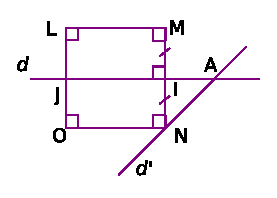
\includegraphics[width=4cm]{programme2}
  \end{minipage} \\
\end{exercice}


\begin{exercice}
Trace une droite $d$ et place un point $R$ qui n'appartient pas à $d$ ;

Construis un carré de sommet $R$, ayant pour axe de symétrie la droite $d$. Combien y a‑t‑il de solutions ?

\end{exercice}


%%%%%%%%%%%%%%%%%%%%%%%%%%%%%%%%%%%%%%%%%%%%%%%%%%%%%%%%%%%%%%%%%

\serie{quadrilatères mélangés…}

\begin{exercice}[Reconnaître]
Quelle est la nature de chaque quadrilatère $ABCD$ :
\begin{center} 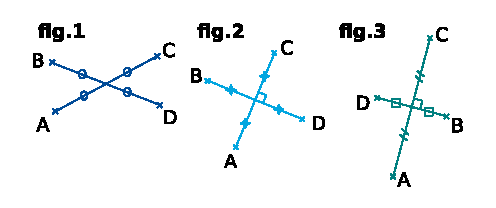
\includegraphics[width=6.8cm]{quadABCD2} \end{center}
\end{exercice}


\begin{exercice}[Constructions]
Construis le rectangle $MODE$ et le losange $CHUT$ :

\qquad 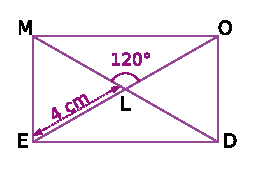
\includegraphics[width=3.4cm]{quadDEMO} \qquad 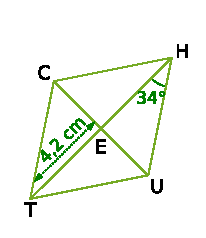
\includegraphics[width=2.5cm]{quadCHTU}
\end{exercice}



\begin{exercice}
Pour chacun des quadrilatères suivants, fais d’abord un croquis puis construis :
\begin{enumerate}
 \item Le rectangle $MANU$ tel que 
 
 $MN = 9$ cm et $MA = 5$ cm ;
 \item Le losange $OURS$ tel que 
 
 $OR = 8$ cm et $US = 6$ cm ;
 \item Le rectangle $PAUL$ tel que 
 
 $PA = 8$ cm et $\widehat{LAU} = 53^\circ$. 
 
 Rédige le programme de construction correspondant.
 \end{enumerate}
\end{exercice}


\begin{exercice}[Une enveloppe plus grande]
\vspace{1em}
\begin{minipage}[c]{0.50\linewidth}
Construis une figure trois fois plus grande en utilisant uniquement ta règle non graduée et ton compas.
 \end{minipage} \hfill%
 \begin{minipage}[c]{0.42\linewidth}
  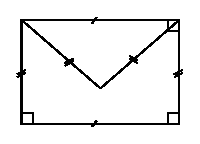
\includegraphics[width=2.6cm]{enveloppe}
  \end{minipage} \\
\end{exercice}


%%%%%%%%%%%%%%%%%%%%%%%%%%%%%%%%%%%%%%%%%%%%%%%%%%%%%%%%%%%%%%%%%
\vspace{1em}
\serie{cercles}

\begin{exercice}[Deux droites sécantes et un cercle]
 \begin{enumerate}
  \item Trace deux droites $d$ et $d'$ sécantes en $O$ sans qu'elles soient perpendiculaires. Place un point $A$ sur $d$. Trace le cercle de centre $O$ et de rayon $OA$. Il recoupe $d$ en $A'$ et $d'$ en $B$ et $B'$ ;
  \item Quelle semble être la nature du quadrilatère $ABA'B'$ ? Et si $d$ et $d'$ sont perpendiculaires ?
  \end{enumerate}
\end{exercice}


\begin{exercice}[Avec des cercles]
\vspace{1em}
Trace deux cercles concentriques de centre $O$. En te servant uniquement d'une règle non graduée, trace un parallélogramme de centre $O$ dont deux sommets appartiennent à l'un des cercles et les deux autres à l'autre cercle.
\end{exercice}


